\documentclass[letterpaper,11pt]{exam}
\usepackage[font=small, labelfont=bf]{caption}
\usepackage{amssymb,amsmath,amsthm,mathtools}
\usepackage{hyperref}
\usepackage{enumitem}
\usepackage{xcolor}
\usepackage{pdfpages}
\usepackage{amsmath}

\usepackage{graphicx}
\usepackage{subcaption}

\usepackage{booktabs}
\usepackage{caption}

\usepackage{pythontex}
\usepackage{listings}
\usepackage{color}
\usepackage{floatflt}
\usepackage{listings}
\usepackage{xcolor}
\usepackage{ulem}

\setlength{\parskip}{1em}  % Space between paragraphs

\definecolor{dkgreen}{rgb}{0,0.6,0}
\definecolor{gray}{rgb}{0.5,0.5,0.5}
\definecolor{mauve}{rgb}{0.58,0,0.82}

\lstset{frame=tb,
  language=Java,
  aboveskip=3mm,
  belowskip=3mm,
  showstringspaces=false,
  columns=flexible,
  basicstyle={\footnotesize\ttfamily},
  numbers=none,
  numberstyle=\tiny\color{gray},
  keywordstyle=\color{blue},
  commentstyle=\color{dkgreen},
  stringstyle=\color{mauve},
  breaklines=true,
  breakatwhitespace=true,
  tabsize=4,
  frame=none
}

\lstset{
    language=C++,
    basicstyle=\ttfamily\footnotesize,
    keywordstyle=\color{blue},
    commentstyle=\color{gray},
    stringstyle=\color{red},
    % numbers=left,
    % numberstyle=\tiny\color{gray},
    stepnumber=1,
    numbersep=5pt,
    showspaces=false,
    showstringspaces=false,
    breaklines=true,
    frame=none,
    captionpos=b
}

\newcommand{\num}{4}
\newcommand{\topic}{Homework \num, Parallel VLSI Wire Routing via MPI}
\newcommand{\coursenum}{15-418/15-618}
\newcommand{\coursename}{\coursenum\ Parallel Computer Architecture and Programming}
\newcommand{\fullname}{Siqi Guo}
\newcommand{\andrew}{AndrewID: siqiguo}
\setlength{\parindent}{0pt} %don't indent first line of paragraph

\definecolor{lightblue}{rgb}{0.2, 0.7, 1} % Light blue in RGB
\hypersetup{
    colorlinks=true,        % Enable colored links (no boxes)
    linkcolor=lightblue,    % Color of internal links
    citecolor=lightblue,    % Color of citation links
    urlcolor=lightblue      % Color of external hyperlinks
}

\pagestyle{headandfoot}
\runningheader{\fullname}{\coursenum\ \textbf{\topic}}{\andrew}
\firstpagefooter{}{\thepage}{}
\runningfooter{}{\thepage}{}
\extrawidth{.5in}\extraheadheight{-.25in}

\begin{document}

\begin{center}
    {\LARGE\coursename\par}
    {\Large\topic\par}
    \fullname (\andrew) \hfill \today
\end{center}
\printanswers

\vspace{-0.2cm}
Use MPI to write a message passing version of the same application as the previous assignment. (Wire Routing under message-passing programming models (only have PRIVATE address spaces).)
\vspace{-0.6cm}

\begin{itemize}[itemsep=0.1pt]
    \item Learn how to compile and run MPI binaries on the same host and across the nodes of a cluster.
    \item Evaluate where optimizations are most valuable.
\end{itemize}

\vspace{-0.8cm}
\begin{quote}
    \textbf{Notes:}

    Sending messages is relatively expensive, experienced MPI programmers generally try to structure their code to avoid frequent communication
\end{quote}

\vspace{-0.5cm}
At the very end, it turns out that machine 28 is a problem where \texttt{perf} is not installed. See 2024 Fall Piazza @368

\begin{questions}
    \question
    \subsection*{[40 points] Design and performance debugging for the message-passing approach.}

    % \begin{enumerate}[label=\roman*.]
    %     \item First, let's visualize the VLSI wire routing.

    %           \begin{figure}[h]
    %               \begin{minipage}{0.3\textwidth}
    %                   \centering
    %                   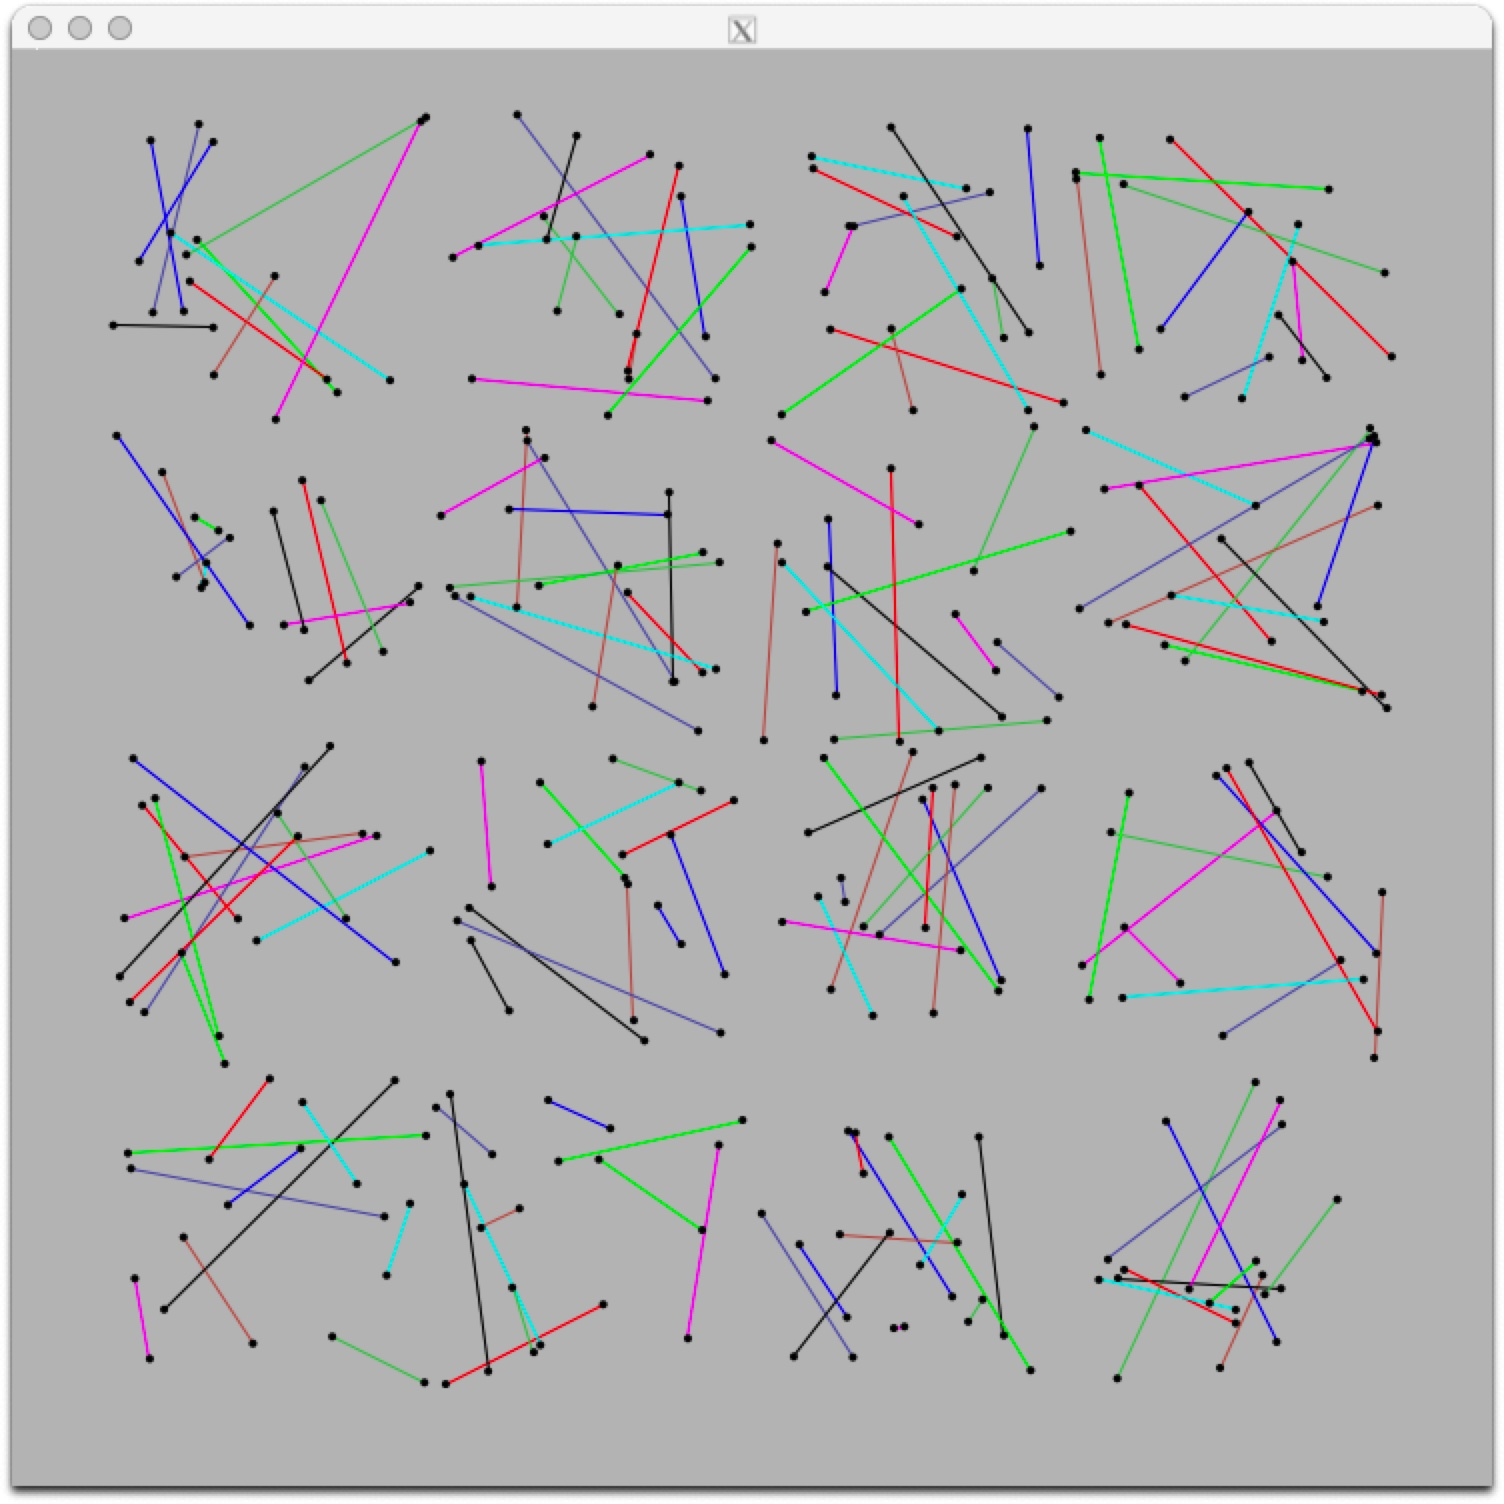
\includegraphics[width=\textwidth]{img/easy_4096.jpg}
    %                   \label{fig:question1a}
    %                   \subcaption{\texttt{java WireGrapher ./inputs/timeinput/easy\_4096.txt}}
    %               \end{minipage}
    %               \hspace{0.2cm}
    %               \begin{minipage}{0.3\textwidth}
    %                   \centering
    %                   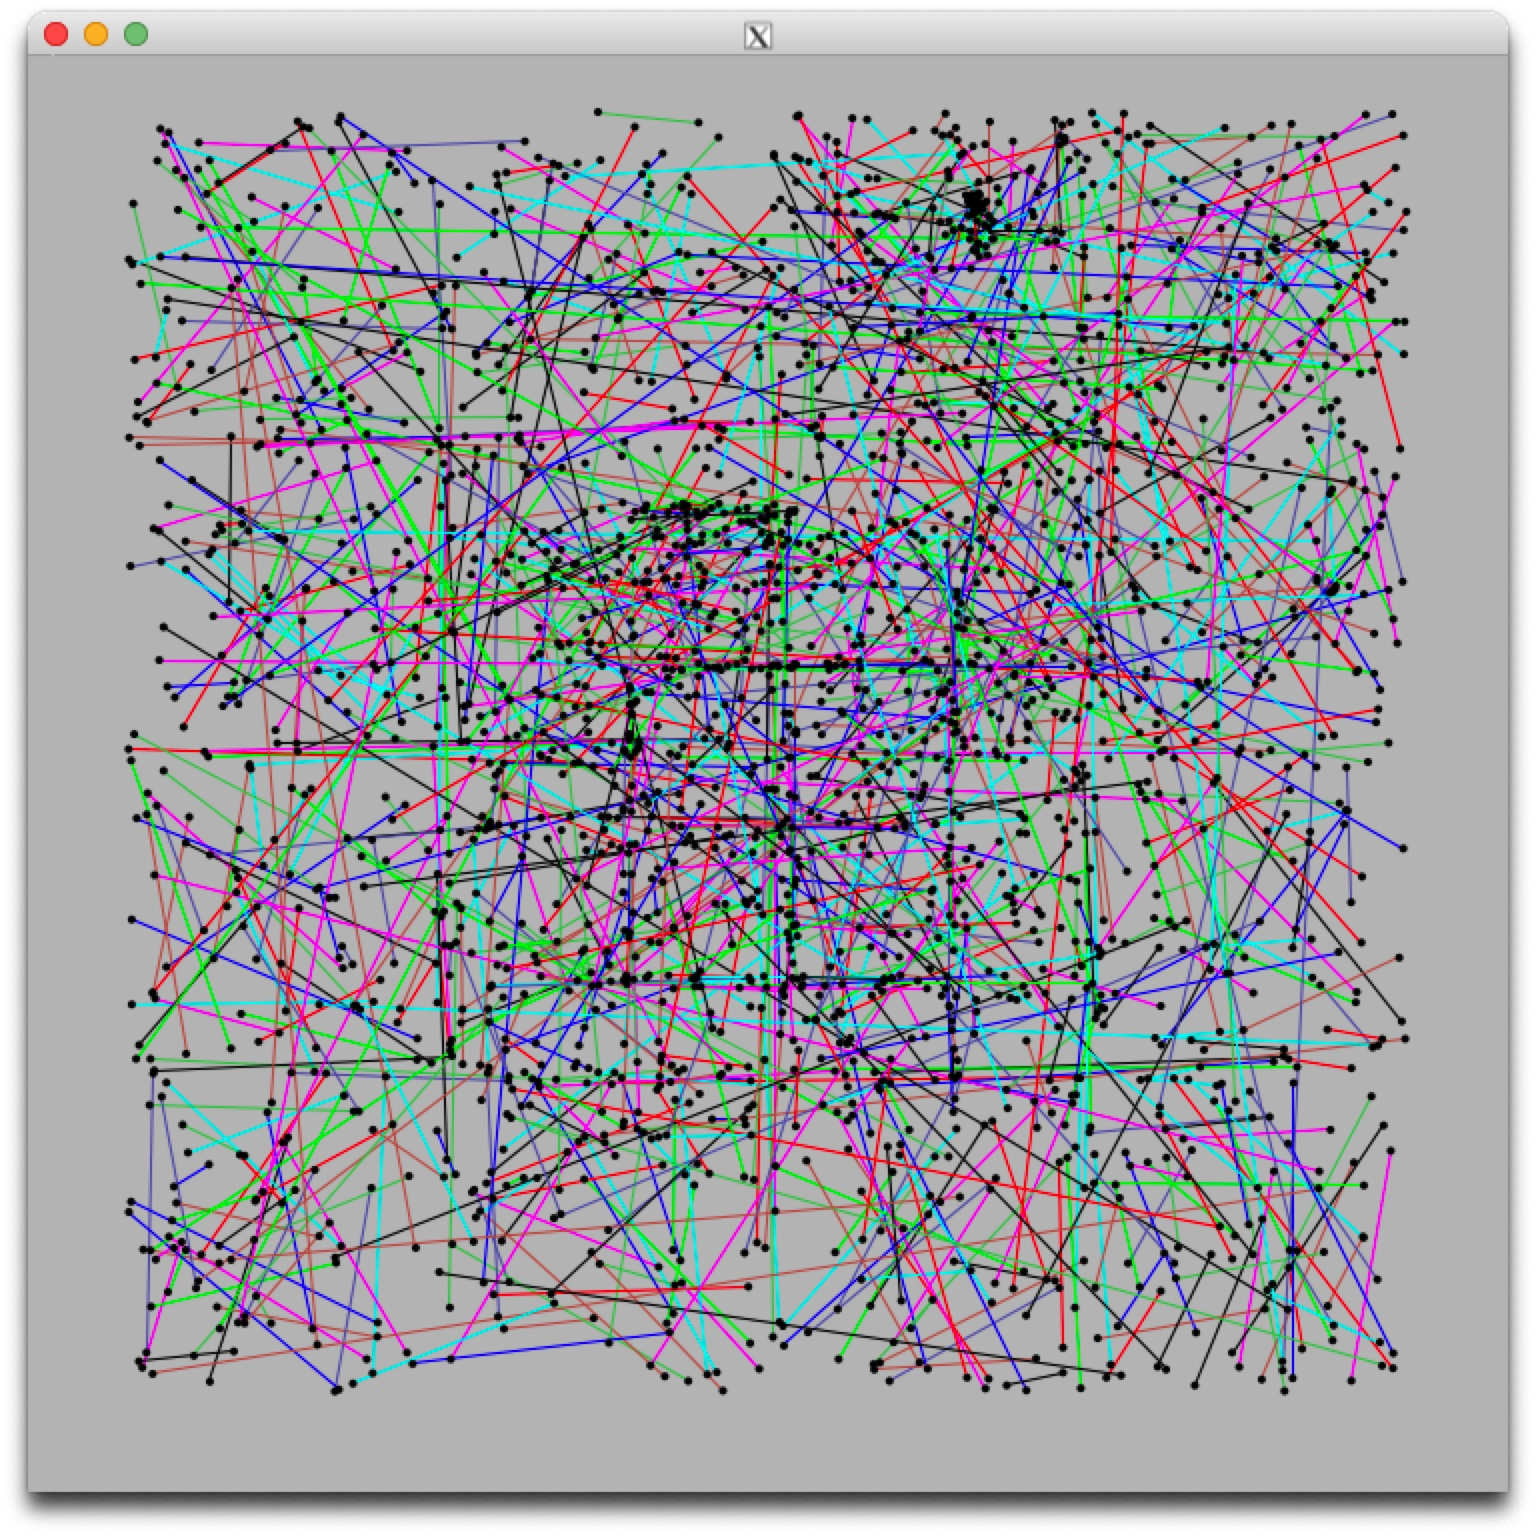
\includegraphics[width=\textwidth]{img/hard_4096.jpg}
    %                   \label{fig:question1b}
    %                   \subcaption{\texttt{java WireGrapher ./inputs/timeinput/hard\_4096.txt}}
    %               \end{minipage}
    %               \hspace{0.2cm}
    %               \begin{minipage}{0.3\textwidth}
    %                   \centering
    %                   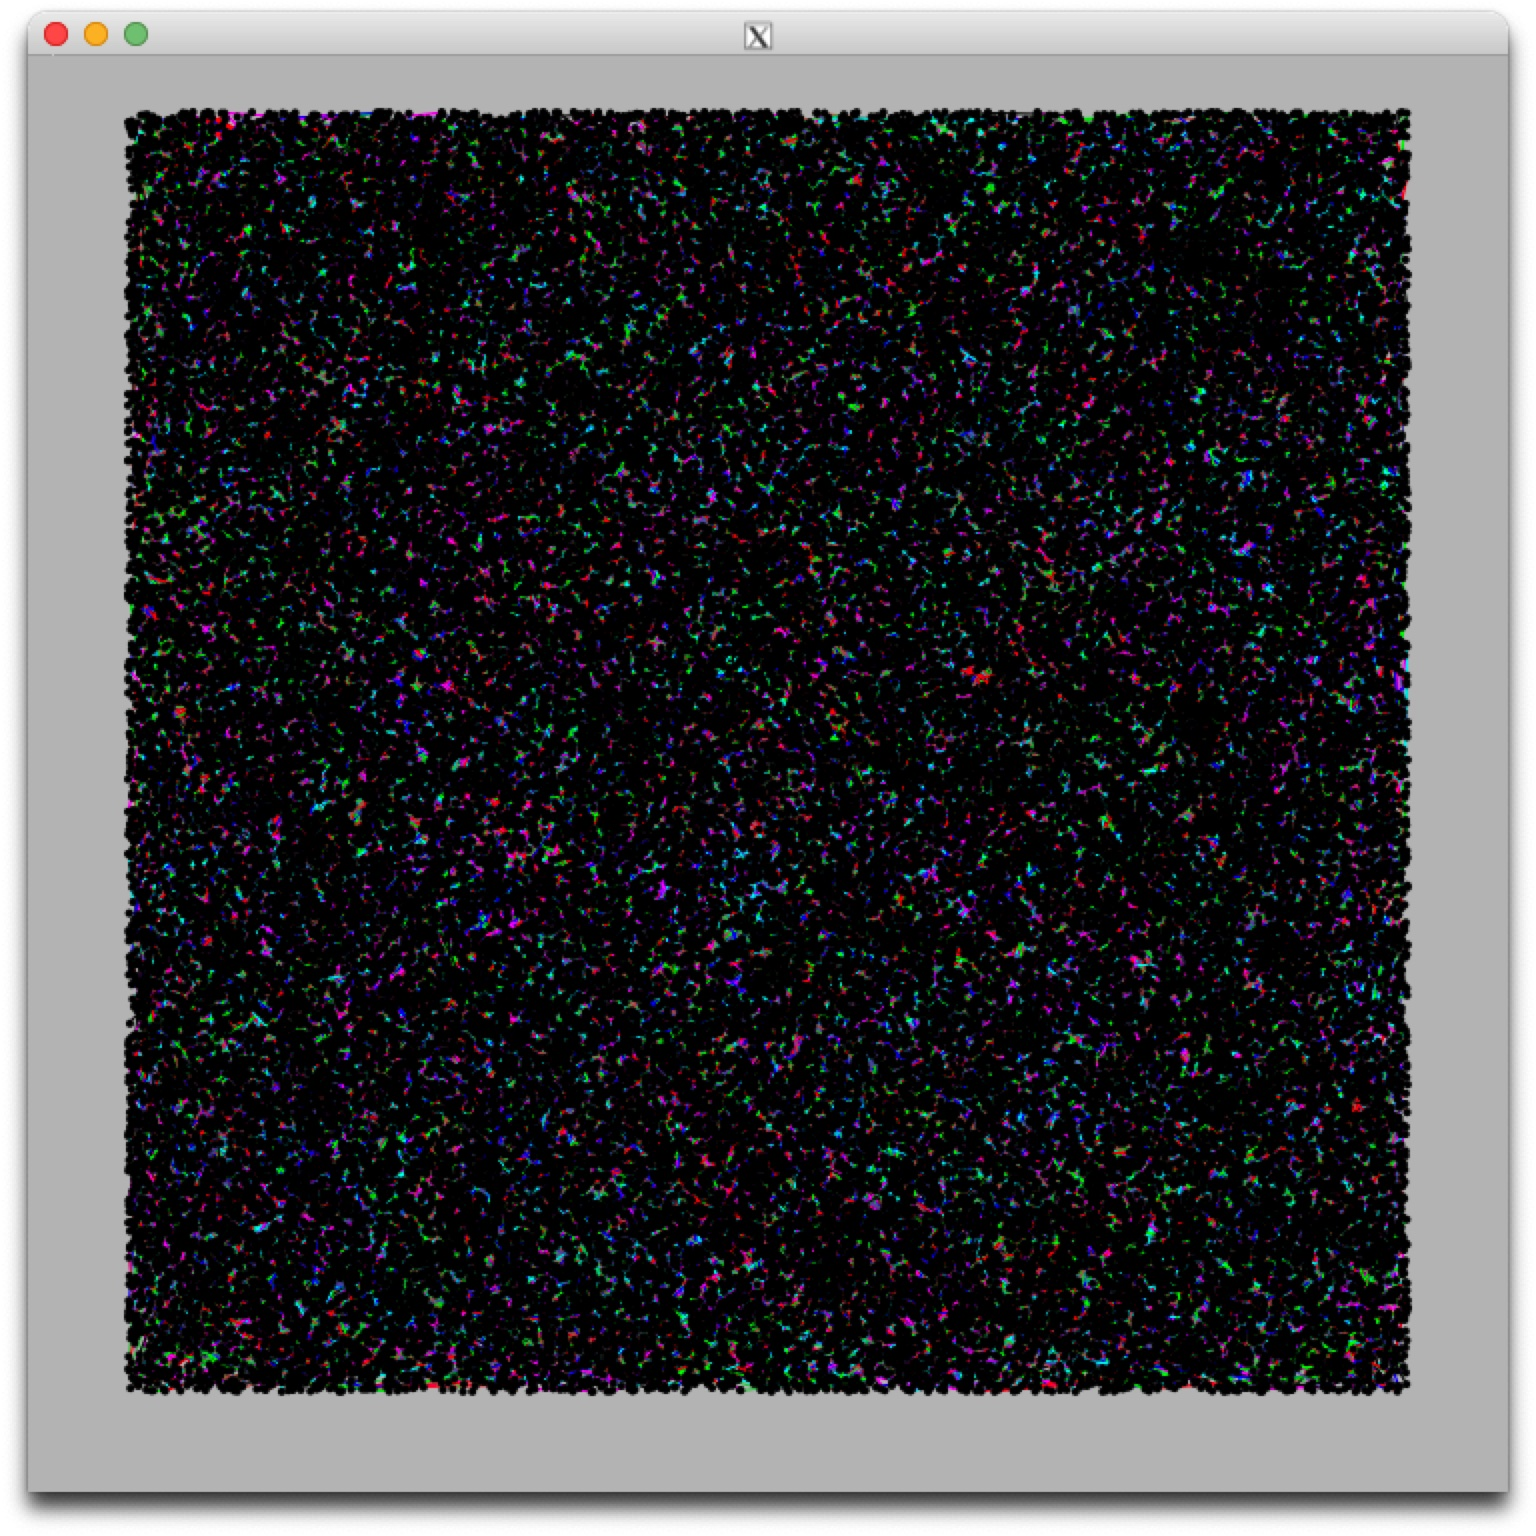
\includegraphics[width=\textwidth]{img/extreme_4096.jpg}
    %                   \label{fig:question1b}
    %                   \subcaption{\texttt{java WireGrapher ./inputs/timeinput/extreme\_4096.txt}}
    %               \end{minipage}

    %               \begin{minipage}{0.3\textwidth}
    %                   \centering
    %                   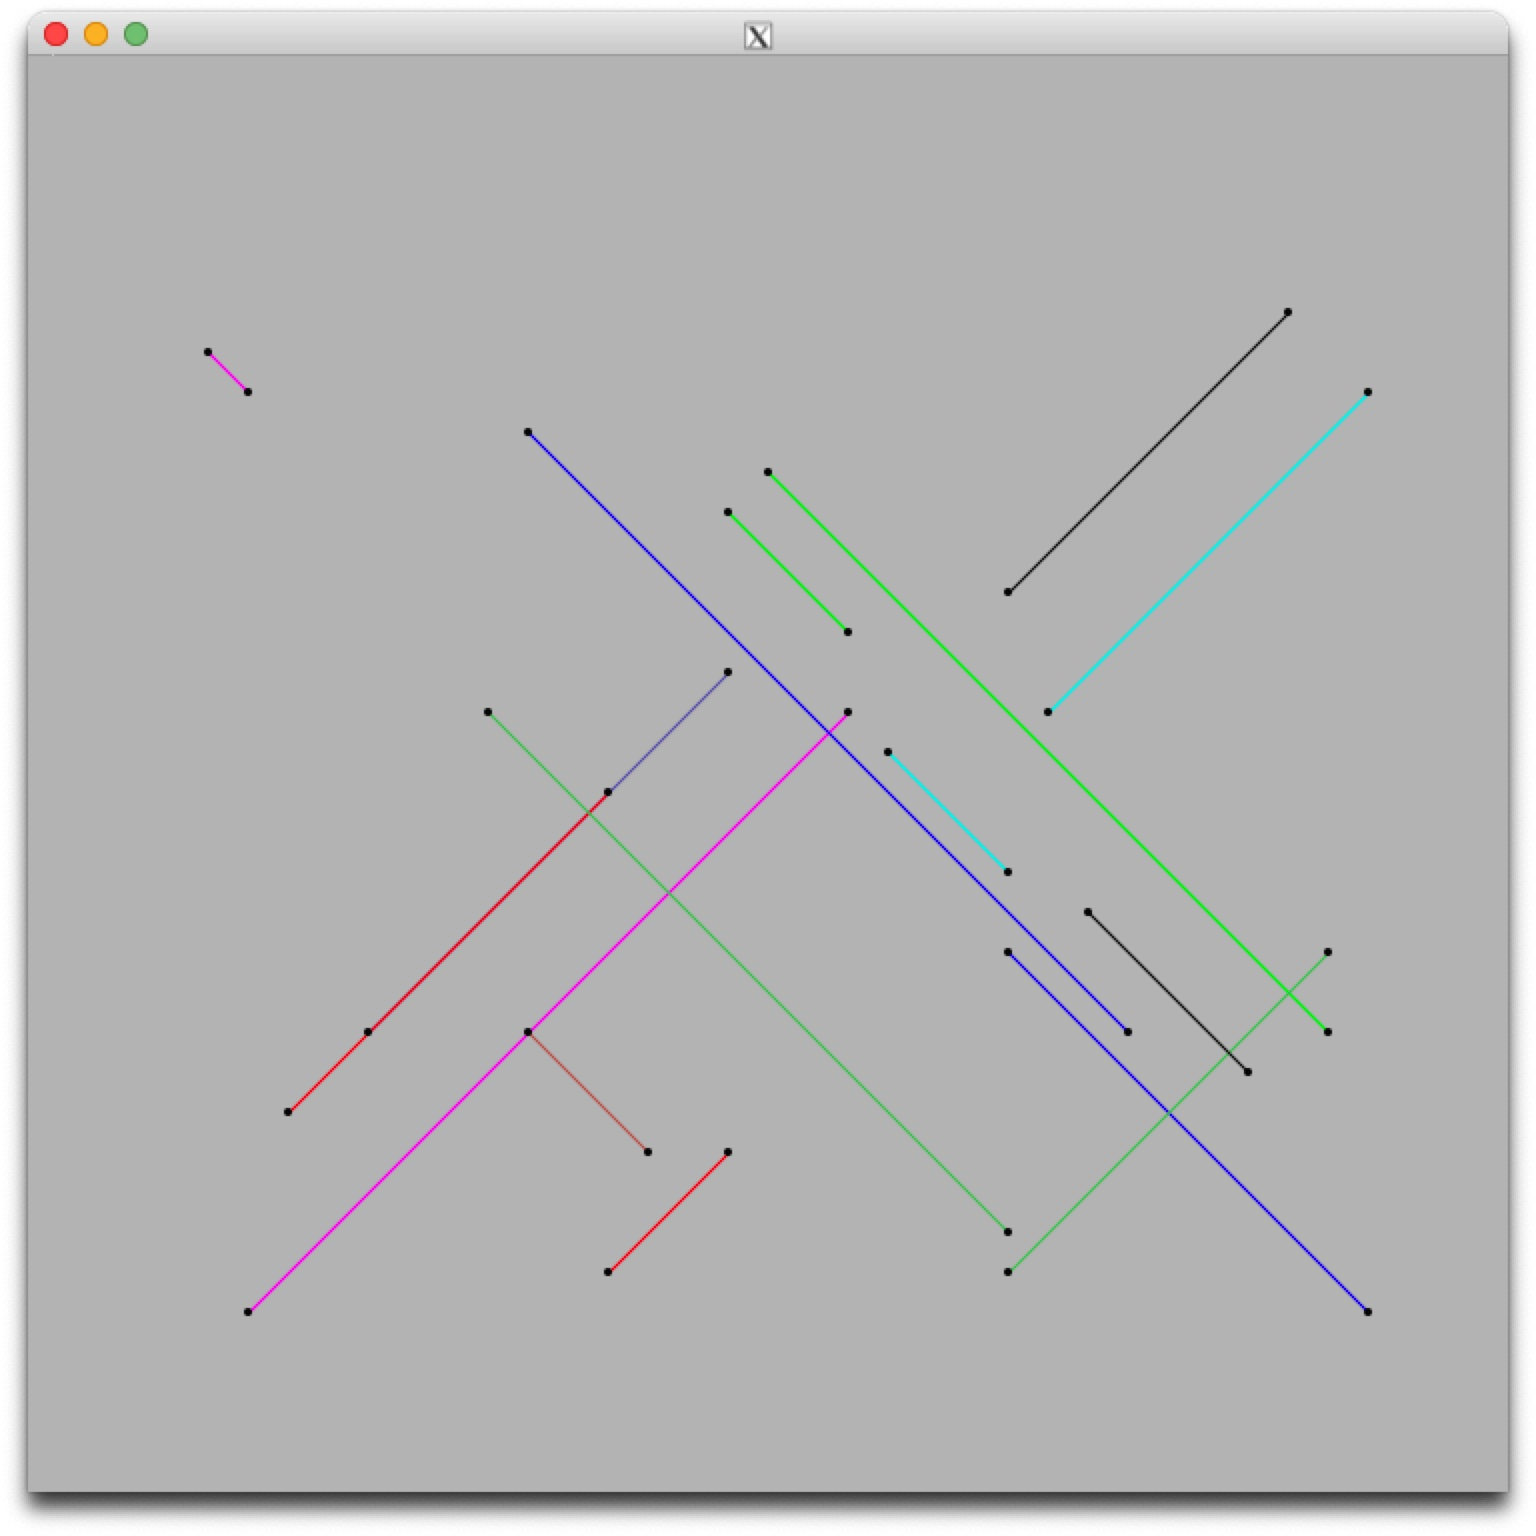
\includegraphics[width=\textwidth]{img/circuit_32x32_16.jpg}
    %                   \label{fig:question1b}
    %                   \subcaption{\scriptsize\texttt{java WireGrapher ./inputs/timeinput/circuit\_32x32\_16.txt}}
    %               \end{minipage}
    %               \hspace{0.2cm}
    %               \begin{minipage}{0.3\textwidth}
    %                   \centering
    %                   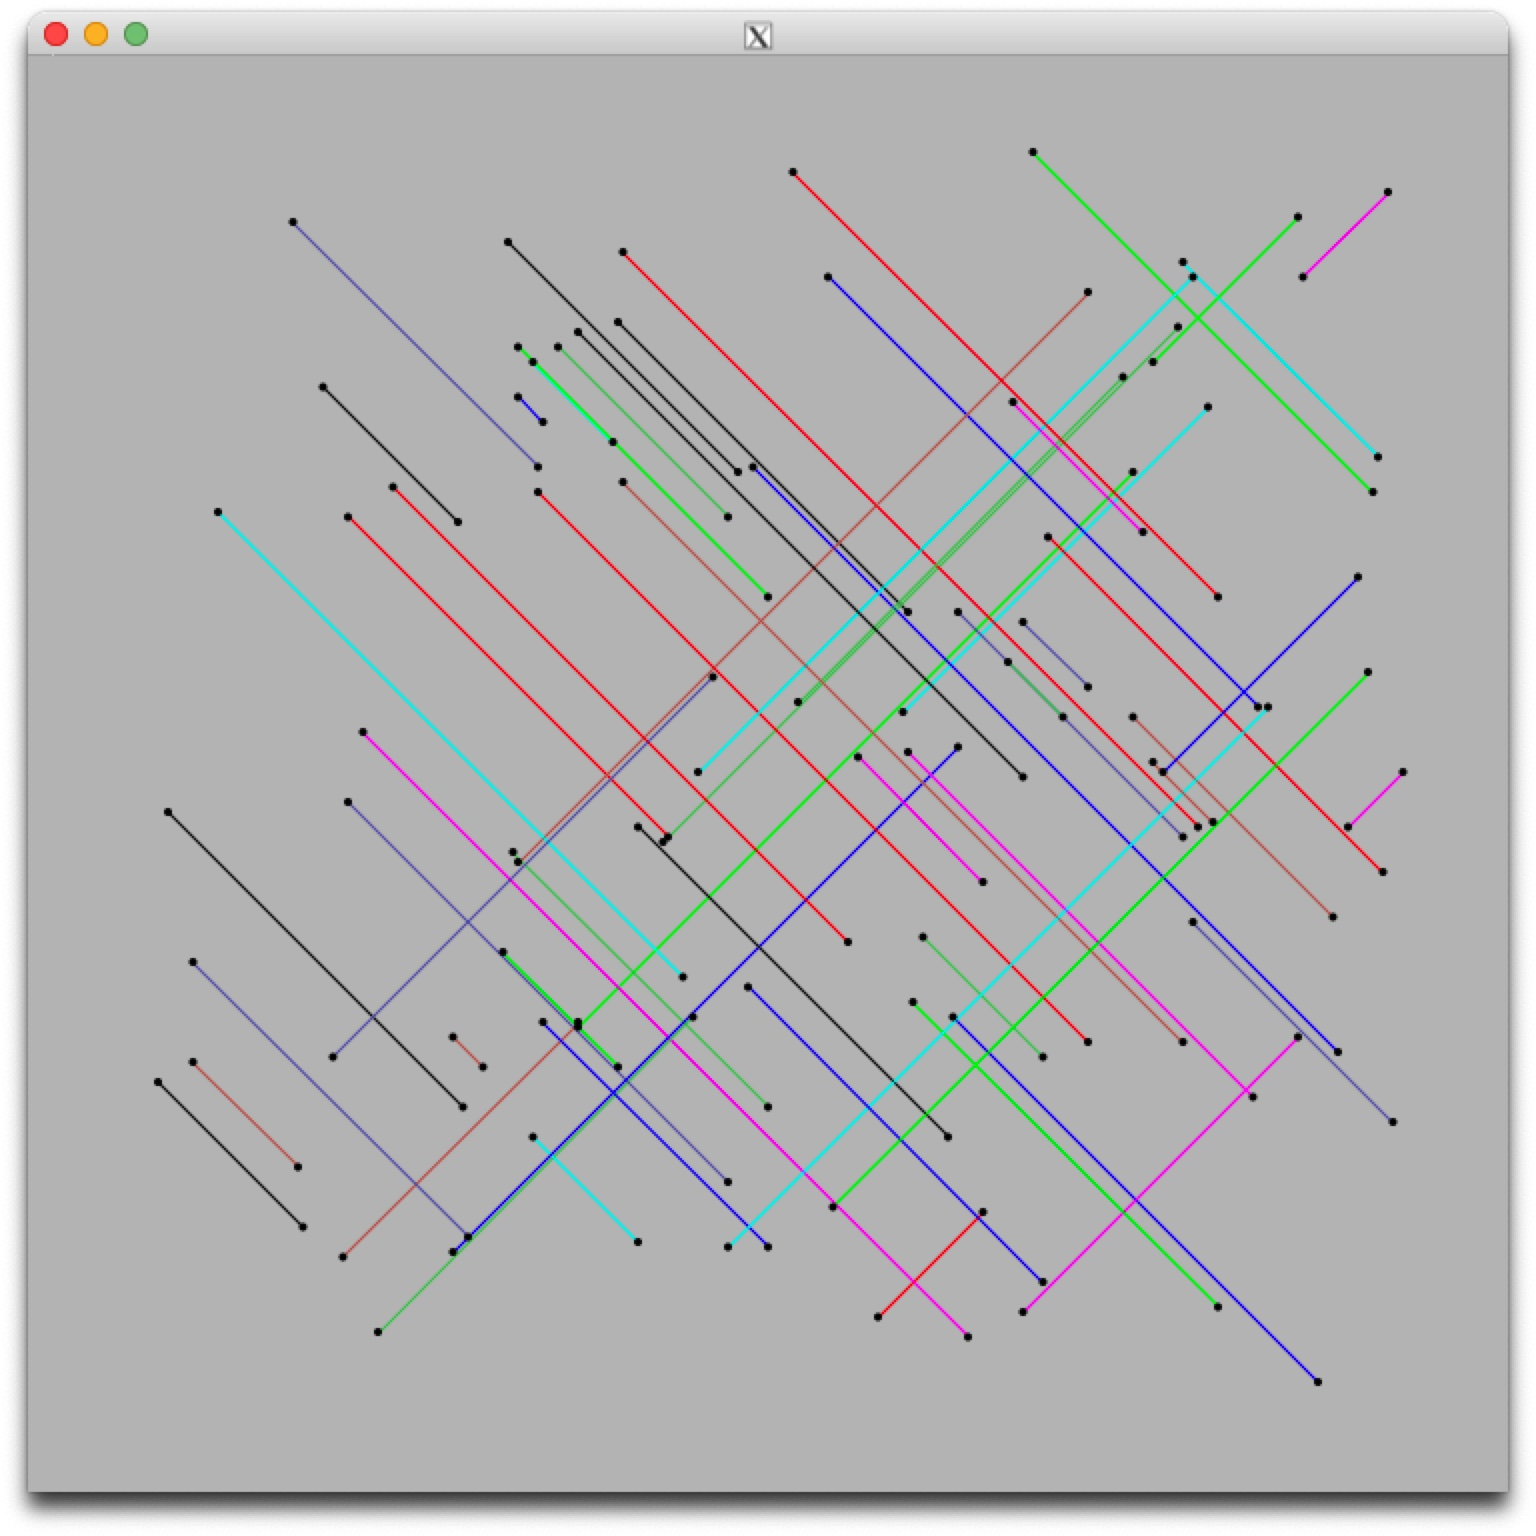
\includegraphics[width=\textwidth]{img/circuit_256x256_64.jpg}
    %                   \label{fig:question1b}
    %                   \subcaption{\scriptsize\texttt{java WireGrapher ./inputs/timeinput/circuit\_256x256\_64.txt}}
    %               \end{minipage}
    %               \hspace{0.2cm}
    %               \begin{minipage}{0.3\textwidth}
    %                   \centering
    %                   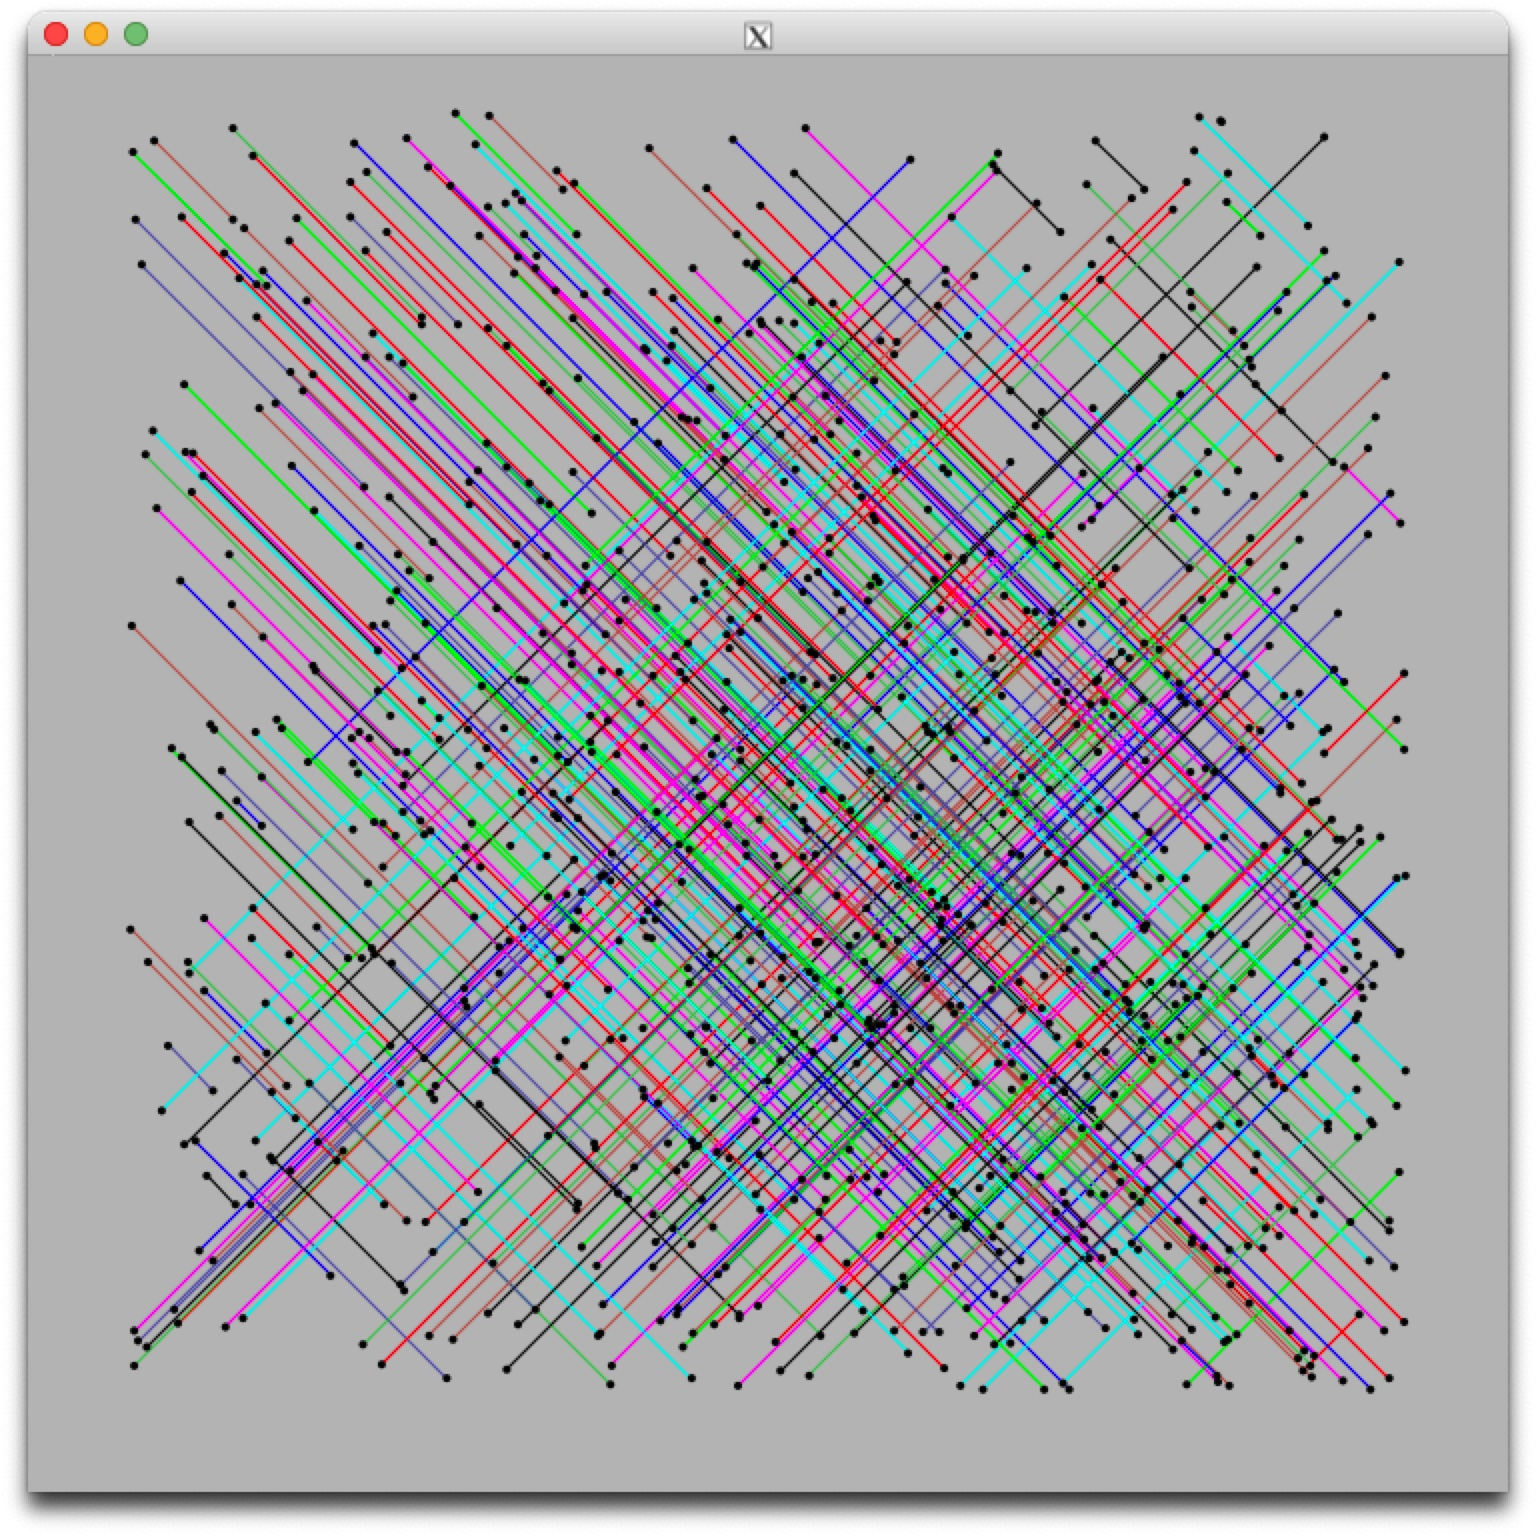
\includegraphics[width=\textwidth]{img/circuit_1024x1024_512.jpg}
    %                   \label{fig:question1b}
    %                   \subcaption{\scriptsize\texttt{java WireGrapher ./inputs/timeinput/circuit\_1024x1024\_512.txt}}
    %               \end{minipage}
    %           \end{figure}
    %           \vspace{0.5cm}

    %           This problem requires us to minimize the overall total cost (the sum of the squares over all matrix elements),
    %           while speedup the programs, taking advantage of parallelism across multiple processor cores.

    %     \item The implementation of \texttt{compute\_cost()} has been completed and passed the correctness test.
    % \end{enumerate}

    \begin{enumerate}[label=\roman*.]
        \item Similar to the OpenMP implementation. After implementing the Across-Wire MPI paralleled program, we have correctness test results attached at the end of the report.
        \item The pseudocode provided.

              \begin{lstlisting}
// Variable Declaration ...
MPI_Init(&argc, &argv);                 // Initialize MPI
MPI_Comm_rank(MPI_COMM_WORLD, &pid);    // Get process rank
MPI_Comm_size(MPI_COMM_WORLD, &nproc);  // Get total number of processes

parse_arguments(...);
initialize_routing(...);

MPI_Bcast(&num_wires, 1, MPI_INT, ROOT, MPI_COMM_WORLD);
MPI_Bcast(&dim_y, 1, MPI_INT, ROOT, MPI_COMM_WORLD);
MPI_Bcast(&dim_x, 1, MPI_INT, ROOT, MPI_COMM_WORLD);
initialize_receiver_vector_size(...);

// MPI_Bcast only work on contiguous memory buffers.
MPI_Bcast(wires.data(), num_wires * sizeof(Wire), MPI_BYTE, ROOT, MPI_COMM_WORLD);
MPI_Bcast(flat_occupancy.data(), dim_y * dim_x * sizeof(int), MPI_BYTE, ROOT, MPI_COMM_WORLD);

// All processes must wait until the broadcast is complete before proceeding to the next step.
If pid is not ROOT
    For each row in occupancy grid
        Copy data from flat_occupancy to 2D occupancy array
    End For
End If

// Calculate work span for each process
Determine work span based on process rank and total wires
Adjust work span for edge cases (e.g., remainder wires)


For each simulated annealing iteration
    For wires assigned to this process (from startIndex to endIndex)
        Perform routing algorithms
    End For
End For

// send data to root process
if (pid != ROOT) {
    MPI_Send(&wires[startIndex], workSpan * sizeof(Wire), MPI_BYTE, ROOT, TAG, MPI_COMM_WORLD);
} else {
    MPI_Status status;
    for (int source = 1; source < nproc; source++) {
        MPI_Recv(&wires[source * workSpan], workSpan * sizeof(Wire), MPI_BYTE, source, TAG, MPI_COMM_WORLD,
                    &status);
    }
}
// This is another synchronization point where the root process must wait for all sends to complete before it can continue.

// Update occupancy grid on ROOT process
If pid is ROOT
    Update occupancy grid with received data
End If

// Cleanup
MPI_Finalize();
        \end{lstlisting}
              % \item The implementation of \texttt{clampedExpVector()} should work with any combination of input
              %       array size N and vector width W.
              % \item Run \texttt{./vrun -s 10000} and sweep the vector width over the values {2, 4, 8, 16, 32}.
              %       Record the resulting vector utilization.

              %       \begin{table}[ht]
              %           \centering
              %           \scriptsize
              %           \begin{tabular}{|c|c|c|c|c|c|}
              %               \hline
              %               VECTOR\_WIDTH W           & 2            & 4            & 8            & 16           & 32           \\ \hline
              %               Total Vector Instructions & 276613       & 141698       & 71238        & 35628        & 17787        \\ \hline
              %               Vector Utilization        & 89.066132 \% & 88.370866 \% & 88.216787 \% & 88.211344 \% & 88.212072 \% \\ \hline
              %           \end{tabular}
              %           \caption{Vector Utilization for Different Vector Widths}
              %       \end{table}

              %       The vector utilization decreases as W increases a bit, but the difference is not significant. The degree of sensitivity the utilization has on the vector width is not very high. \\
              %       The higher W is, the more vector instructions are executed.

              % \item \texttt{arraySumVector()} has been implemented, and the results passed the correctness test as follows.

              %       \includegraphics*[width=0.65\textwidth]{./prog2\_vecintrin/arraySumVector.jpg}
    \end{enumerate}

    \question
    \subsection*{[15 points] Experimental results from the GHC machines}
    % \begin{enumerate}[label=\roman*.]
    %     \item First,
    % \end{enumerate}

    \question
    \subsection*{\sout{[20 points] Experimental results from the PSC machines}}
    % \begin{enumerate}[label=\roman*.]
    % \end{enumerate}

    % \question
    % \subsection*{Problem 4: Iterative Square Root (10 points)}

    % \begin{enumerate}[label=\roman*.]
    %     \item The sqrt program has been built and run. The speedup due to SIMD (no
    %           tasks) parallelization is 4.77x. The speedup due to multi-core parallelization
    %           is 34.69x.

    %     \item The speedup under different scenarios is as follows.

    %           \begin{table}[ht]
    %               \centering
    %               \scriptsize
    %               \begin{tabular}{|c|c|c|c|}
    %                   \hline
    %                   Case               & Random & initGood & initBad \\ \hline
    %                   SIMD Speedup       & 4.77x  & 6.88x    & 0.95x   \\ \hline
    %                   Multi-Core Speedup & 34.68x & 50.16x   & 6.89x   \\ \hline
    %               \end{tabular}
    %               \caption{Speedup under Different Scenarios}
    %           \end{table}

    %           The \texttt{initGood()} change the value to 2.999. The initialized value of 2.999 could result in the maximum
    %           iteration, and accelerate the paralleled computation to the largest extent. This
    %           modification improves both SIMD and multi-core speedup.

    %           The \texttt{initBad()} change the value to 1.0. The value around 1.0 results in the minimum iteration and the
    %           least absolute computation time. There is not much time to decrease with
    %           parallelism. This modification decreases SIMD and multi-core speedup.

    %           %   \includegraphics*[width=0.65\textwidth]{./prog4\_isqrt/output\_log/speedup_vs_thread_count.png}
    % \end{enumerate}

    % \newpage

    % \question

    % \subsection*{Problem 5: BLAS saxpy (10 points)}

    % The saxpy routine in the BLAS (Basic Linear Algebra Subproblems) library that is
    % widely used (and heavily optimized) on many systems.

    % The \textbf{saxpy} function computes the operation:
    % $\mathbf{r} = a \mathbf{x} + \mathbf{y}$
    % where $a$ is a scalar, and $\mathbf{r}, \mathbf{x}, \mathbf{y}$ are vectors of size $N$ containing single-precision floating-point values.
    % The term \textbf{saxpy} is an acronym for \textbf{"single-precision a x plus y"}.

    % \begin{enumerate}[label=\roman*.]
    %     \item The speedup due to SIMD parallelization is 1x. The speedup from ISPC with tasks is 1.03x.

    %           \captionsetup{font=small, labelfont=bf}
    %           \begin{table}[h!]
    %               \centering
    %               \caption{SAXPY Performance Comparison}
    %               \begin{tabular}{@{}lccc@{}}
    %                   \toprule
    %                   \textbf{Method} & \textbf{Time (ms)} & \textbf{Bandwidth (GB/s)} & \textbf{GFLOPS} \\
    %                   \midrule
    %                   SAXPY Serial    & 11.238             & 26.520                    & 1.780           \\
    %                   SAXPY Streaming & 11.238             & 26.520                    & 1.780           \\
    %                   SAXPY ISPC      & 11.246             & 26.500                    & 1.778           \\
    %                   SAXPY Task ISPC & 10.920             & 27.291                    & 1.831           \\
    %                   \midrule
    %                   \multicolumn{4}{l}{(1.00x speedup from streaming)}                                 \\
    %                   \multicolumn{4}{l}{(1.00x speedup from ISPC)}                                      \\
    %                   \multicolumn{4}{l}{(1.03x speedup from task ISPC)}                                 \\
    %                   \bottomrule
    %               \end{tabular}
    %               \label{tab:saxpy-performance}
    %           \end{table}

    %           I do not think we could achieve linear speedup as the memory bandwidth could be the bottleneck.

    %     \item One value is loaded from vector x \texttt{(N x sizeof(float))}. One value is loaded from vector y \texttt{(N x sizeof(float))}.
    %           One value is written to the result vector  r \texttt{(N x sizeof(float))}.
    %           However, result should be stored in the cache, thus a cache miss will lead to 2 N (read from memory to cache, then back to memory).

    %     \item In addition to the memory bandwidth, the performance of SAXPY might be also limited by poor cache utilization, high cache misses, low pre-fetching efficiency, and the latency of FP operations or DRAM.
    %     \item Improve the performance of saxpy by reducing the memory requirement (modify \texttt{saxpyStreaming()}).
    %           \captionsetup{font=small, labelfont=bf}
    %           \begin{table}[h!]
    %               \centering
    %               \caption{SAXPY Performance Comparison After Streaming}
    %               \begin{tabular}{@{}lccc@{}}
    %                   \toprule
    %                   \textbf{Method} & \textbf{Time (ms)} & \textbf{Bandwidth (GB/s)} & \textbf{GFLOPS} \\
    %                   \midrule
    %                   SAXPY Serial    & 11.280             & 26.421                    & 1.773           \\
    %                   SAXPY Streaming & 8.209              & 36.302                    & 2.436           \\
    %                   SAXPY ISPC      & 11.122             & 26.797                    & 1.798           \\
    %                   SAXPY Task ISPC & 10.900             & 27.342                    & 1.835           \\
    %                   \midrule
    %                   \multicolumn{4}{l}{(1.37x speedup from streaming)}                                 \\
    %                   \multicolumn{4}{l}{(1.01x speedup from ISPC)}                                      \\
    %                   \multicolumn{4}{l}{(1.03x speedup from task ISPC)}                                 \\
    %                   \bottomrule
    %               \end{tabular}
    %               \label{tab:saxpy_comparison}
    %           \end{table}
    % \end{enumerate}
    \newpage


    \subsection*{Correctness Tests}
    \begin{lstlisting}[basicstyle=\tiny\ttfamily]
siqiguo@ghc56:~/private/15-618-Parallel-Computing/asst4/code$ ./checker.pl

--------------
Running tests on ghc56.ghc.andrew.cmu.edu
--------------

Test : easy with 1 cores
Correctness passed!
Your time : 0.6370366600
Target Time: 0.49
Your cost : 121978
Target Cost: 122050

Test : easy with 2 cores
Correctness passed!
Your time : 0.3346642290
Target Time: 0.31
Your cost : 122405
Target Cost: 122050

Test : easy with 4 cores
Correctness passed!
Your time : 0.2201978630
Target Time: 0.19
Your cost : 123904
Target Cost: 122050

Test : easy with 8 cores
Correctness passed!
Your time : 0.1405227760
Target Time: 0.13
Your cost : 125892
Target Cost: 122050

Test : medium with 1 cores
Correctness passed!
Your time : 10.9571411100
Target Time: 9.52
Your cost : 601215
Target Cost: 601213

Test : medium with 2 cores
Correctness passed!
Your time : 9.9203150420
Target Time: 6.12
Your cost : 612134
Target Cost: 601213

Test : medium with 4 cores
Correctness passed!
Your time : 8.0959574360
Target Time: 4.04
Your cost : 621736
Target Cost: 601213

Test : medium with 8 cores
Correctness passed!
Your time : 6.8566017200
Target Time: 3.41
Your cost : 641197
Target Cost: 601213

Test : hard with 1 cores
Correctness passed!
Your time : 13.4858831170
Target Time: 11.15
Your cost : 1031998
Target Cost: 1032198

Test : hard with 2 cores
Correctness passed!
Your time : 11.2784738400
Target Time: 7.08
Your cost : 1052142
Target Cost: 1032198

Test : hard with 4 cores
Correctness passed!
Your time : 10.8472393710
Target Time: 4.1
Your cost : 1063102
Target Cost: 1032198

Test : hard with 8 cores
Correctness passed!
Your time : 7.5720181200
Target Time: 3.1
Your cost : 1076051
Target Cost: 1032198

Test : extreme with 1 cores
Correctness passed!
Your time : 59.0921018140
Target Time: 46.81
Your cost : 23592484
Target Cost: 23613045

Test : extreme with 2 cores
Correctness passed!
Your time : 30.5852387770
Target Time: 28.95
Your cost : 26268192
Target Cost: 23613045

Test : extreme with 4 cores
Correctness passed!
Your time : 16.0450465490
Target Time: 15.2
Your cost : 29031434
Target Cost: 23613045

Test : extreme with 8 cores
Correctness passed!
Your time : 8.5529003170
Target Time: 11
Your cost : 30714138
Target Cost: 23613045

------------
Score table:
------------
----------------------------------------------------------------------------------------------------------------------------------------------------
| Test Name          | Core Num           | Target Time        | Your Time          | Target Cost        | Your Cost          | Score              |
----------------------------------------------------------------------------------------------------------------------------------------------------
| easy               | 1                  | 0.49               | 0.6370366600       | 122050             | 121978             | 0.769186501762709  |
| easy               | 2                  | 0.31               | 0.3346642290       | 122050             | 122405             | 1                  |
| easy               | 4                  | 0.19               | 0.2201978630       | 122050             | 123904             | 1                  |
| easy               | 8                  | 0.13               | 0.1405227760       | 122050             | 125892             | 1                  |
| medium             | 1                  | 9.52               | 10.9571411100      | 601213             | 601215             | 2                  |
| medium             | 2                  | 6.12               | 9.9203150420       | 601213             | 612134             | 1.2338317833838    |
| medium             | 4                  | 4.04               | 8.0959574360       | 601213             | 621736             | 0.998028962463532  |
| medium             | 8                  | 3.41               | 6.8566017200       | 601213             | 641197             | 0.994661827900367  |
| hard               | 1                  | 11.15              | 13.4858831170      | 1032198            | 1031998            | 2.48037148993481   |
| hard               | 2                  | 7.08               | 11.2784738400      | 1032198            | 1052142            | 1.88323352089275   |
| hard               | 4                  | 4.1                | 10.8472393710      | 1032198            | 1063102            | 1.13392906520381   |
| hard               | 8                  | 3.1                | 7.5720181200       | 1032198            | 1076051            | 1.22820625262846   |
| extreme            | 1                  | 46.81              | 59.0921018140      | 23613045           | 23592484           | 3.16861296606714   |
| extreme            | 2                  | 28.95              | 30.5852387770      | 23613045           | 26268192           | 3.59568637232437   |
| extreme            | 4                  | 15.2               | 16.0450465490      | 23613045           | 29031434           | 3.25344521390159   |
| extreme            | 8                  | 11                 | 8.5529003170       | 23613045           | 30714138           | 3.0752020453903    |
----------------------------------------------------------------------------------------------------------------------------------------------------
|                                                                                                       | Total score:       | 28.8143960018536/40 |
----------------------------------------------------------------------------------------------------------------------------------------------------
    \end{lstlisting}
\end{questions}

\end{document}